
\let\negmedspace\undefined
\let\negthickspace\undefined
\documentclass[journal]{IEEEtran}
\usepackage[a5paper, margin=10mm, onecolumn]{geometry}
%\usepackage{lmodern} % Ensure lmodern is loaded for pdflatex
\usepackage{tfrupee} % Include tfrupee package

\setlength{\headheight}{1cm} % Set the height of the header box
\setlength{\headsep}{0mm}     % Set the distance between the header box and the top of the text

\usepackage{gvv-book}
\usepackage{gvv}
\usepackage{cite}
\usepackage{amsmath,amssymb,amsfonts,amsthm}
\usepackage{algorithmic}
\usepackage{graphicx}
\usepackage{textcomp}
\usepackage{xcolor}
\usepackage{txfonts}
\usepackage{listings}
\usepackage{enumitem}
\usepackage{mathtools}
\usepackage{gensymb}
\usepackage{comment}
\usepackage[breaklinks=true]{hyperref}
\usepackage{tkz-euclide} 
\usepackage{listings}
% \usepackage{gvv}                                        
\def\inputGnumericTable{}                                 
\usepackage[latin1]{inputenc}                                
\usepackage{color}                                            
\usepackage{array}                                            
\usepackage{longtable}                                       
\usepackage{calc}                                             
\usepackage{multirow}                                         
\usepackage{hhline}                                           
\usepackage{ifthen}                                           
\usepackage{lscape}
\begin{document}

\bibliographystyle{IEEEtran}
\vspace{3cm}

\title{1.11.1}
\author{EE24BTECH11020 - Ellanti Rohith}
% \maketitle
% \newpage
% \bigskip
{\let\newpage\relax\maketitle}

\renewcommand{\thefigure}{\theenumi}
\renewcommand{\thetable}{\theenumi}
\setlength{\intextsep}{10pt} % Space between text and floats


\numberwithin{equation}{enumi}
\numberwithin{figure}{enumi}
\renewcommand{\thetable}{\theenumi}


\textbf{Question}:Find a vector $\overrightarrow{r}$ equally inclined to the three axes and whose magnitude is $3\sqrt{3}$ units.\\ \textbf{Solution:} Let $\alpha$ be the angle made by the vector with the axes.  The unit direction vector can be expressed as
   
\begin{align}
\vec{x} &= \myvec{\cos\alpha \\ \cos\alpha \\ \cos\alpha} \\
\implies \norm{\vec{x}} &= 1 \\
\text{or, } \cos\alpha &= \frac{1}{\sqrt{3}} \\
\vec{x} &= \frac{1}{\sqrt{3}} (\hat{i} + \hat{j} + \hat{k})
\end{align}

Given that \(\norm{\vec{r}} = 3\sqrt{3}\), we have:
\begin{align}
\norm{\vec{r}} &= 3\sqrt{3} \\
\vec{x} &= \frac{\vec{r}}{\norm{\vec{r}}} \\
\implies \vec{r} &= \vec{x} \norm{\vec{r}} \\
\text{Thus, the vector } \vec{r} &= (3\hat{i} + 3\hat{j} + 3\hat{k})
\end{align}


\newpage

\begin{figure}[h!]
   \centering 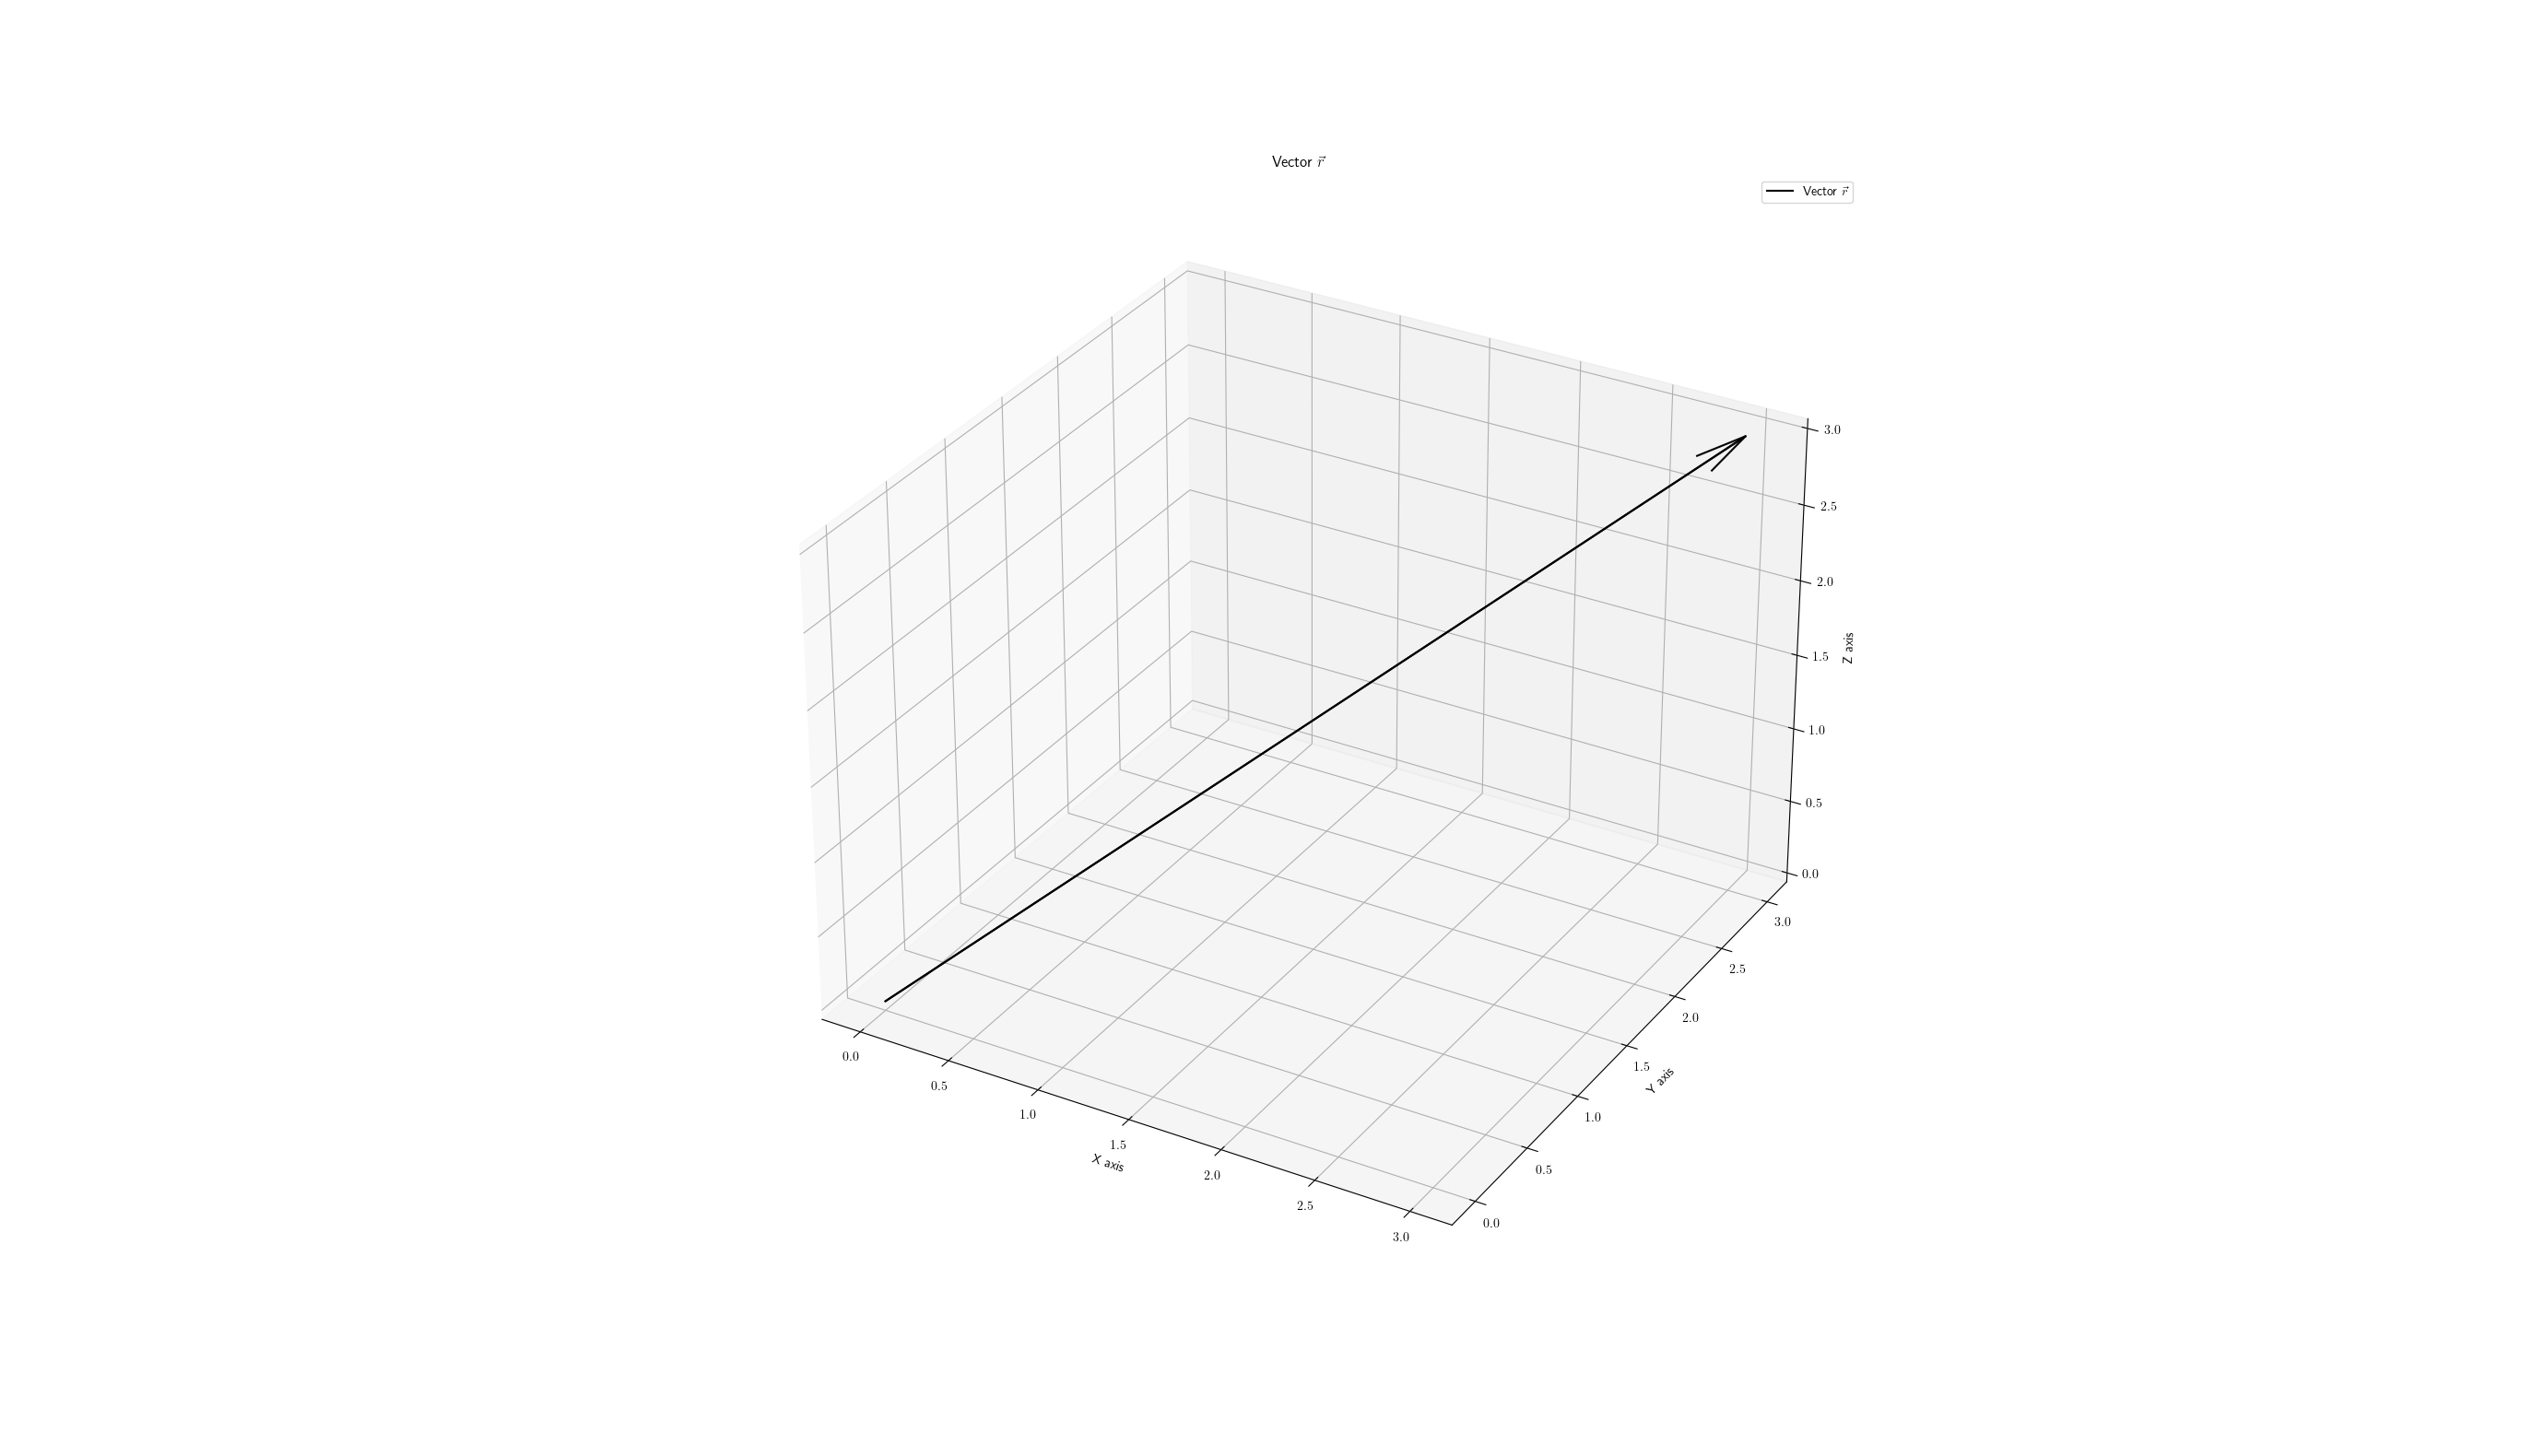
\includegraphics[width=1.1\textwidth]{figs/fig.png}
   \label{Plot of Given Vector}
   \end{figure}
	

\end{document}

